\documentclass{midl}

\usepackage{booktabs}
\usepackage{multirow}
\usepackage{xcolor}

% Tighten layout for short-paper page budget
\setlength{\textfloatsep}{6pt plus 1pt minus 1pt}
\setlength{\intextsep}{6pt plus 1pt minus 1pt}
\setlength{\abovecaptionskip}{3pt}
\setlength{\belowcaptionskip}{2pt}

\jmlrproceedings{MIDL}{Medical Imaging with Deep Learning}
\jmlrpages{}
\jmlryear{2026}

\jmlrworkshop{Short Paper -- MIDL 2026 submission}
\jmlrvolume{-- Under Review}
\editors{Under Review for MIDL 2026}

\title[Post-hoc Entropy Minimization for SSL Segmentation]{Post-hoc Entropy Minimization Improves Semi-Supervised Medical Image Segmentation}

% TODO: fill in author info before submission
\midlauthor{\Name{Author Name1\nametag{$^{1}$}} \Email{author1@example.edu}\\
\Name{Author Name2\nametag{$^{1}$}} \Email{author2@example.edu}\\
\addr $^{1}$ Institution Name}

\begin{document}

\maketitle

% ══════════════════════════════════════════════════════════════════════════════
\begin{abstract}
Semi-supervised learning (SSL) methods for medical image segmentation discard the unlabeled data once training converges, even though the model's predictions still contain residual uncertainty concentrated at organ boundaries.
We show that this residual entropy is structured and exploitable.
\textbf{Post-hoc Entropy Minimization (PEM)} takes any converged SSL checkpoint and fine-tunes it for a few epochs using only entropy minimization on unlabeled data --- no labels, no pseudo-labels, no architectural changes.
Applied on top of publicly released BCP~\cite{bai2023bcp} checkpoints, PEM improves Dice from 82.9 to \textbf{84.0} on Pancreas-CT (20\%), from 87.3 to \textbf{88.9} on LA (5\%), and from 89.4 to \textbf{90.3} on LA (10\%), while reducing 95\% Hausdorff distance by 28\%, 44\%, and 34\% respectively, in under five minutes of fine-tuning.
\end{abstract}

\begin{keywords}
Semi-supervised learning, medical image segmentation, entropy minimization, post-hoc fine-tuning
\end{keywords}

% ══════════════════════════════════════════════════════════════════════════════
\section{Introduction}
\label{sec:intro}

Recent SSL methods for medical image segmentation~\cite{tarvainen2017meanteacher,yu2019uamt,bai2023bcp,liu2024most,assefa2025dycon} share a common property: once training converges, the unlabeled data is abandoned.
Yet the model's predictions on unlabeled volumes still contain residual uncertainty --- in a converged BCP model on Pancreas-CT, only $\sim$5\% of voxels have $\max_c p_{i,c} < 0.99$, and those voxels lie almost entirely on the organ surface.
This boundary-concentrated entropy is an untapped source of self-supervision.

We propose \textbf{Post-hoc Entropy Minimization (PEM)}: take any converged SSL checkpoint, fine-tune for a few epochs on unlabeled data with a single entropy loss --- no labels, no pseudo-labels, no architectural changes, no extra models.
Applied to publicly released BCP checkpoints, PEM consistently improves both Dice and HD95 on three benchmark configurations spanning two datasets.
Entropy minimization itself is classical~\cite{grandvalet2004entropy} and widely used in domain adaptation and SSL classification~\cite{sohn2020fixmatch}, but to our knowledge its use as a post-hoc refinement of converged 3D segmentation checkpoints has not been explored.

% ══════════════════════════════════════════════════════════════════════════════
\section{Method}
\label{sec:method}
\vspace{-2pt}

Let $f_{\theta^*}$ be a segmentation network trained by an SSL method to convergence and let $p_i = \mathrm{softmax}(f_{\theta^*}(\mathbf{x})_i)$ be its softmax output at voxel $i$ on an unlabeled volume $\mathbf{x}\in\mathcal{U}$.
The per-voxel entropy is $H_i = -\sum_c p_{i,c} \log p_{i,c}$, and PEM minimizes its mean over $\mathcal{U}$, optionally restricted to voxels whose top class probability is below a threshold $\tau$:
\begin{equation}
    \mathcal{L}_{\text{PEM}} =
    \frac{1}{|\mathcal{U}|}\sum_{\mathbf{x}\in\mathcal{U}}
    \frac{\sum_{i} m_i\, H_i(\mathbf{x})}{\sum_i m_i + \epsilon},
    \qquad
    m_i = \mathbb{1}[\max_c p_{i,c} < \tau].
    \label{eq:pem}
\end{equation}
$\tau\!=\!1$ recovers full-volume entropy minimization (\textit{full mode}); $\tau\in[0.9,0.99]$ restricts the loss to the small fraction of uncertain boundary voxels (\textit{confident mode}), which we find better when the base model is highly saturated.

\paragraph{Implementation.}
Adam, dataset-dependent low LR ($5\!\times\!10^{-5}$ Pancreas, $1\!\times\!10^{-5}$ LA --- gentler because LA's base model is more confident), gradient clipping (max norm 1.0), and early stopping when test Dice fails to improve for five epochs or drops 0.5\% below baseline.
For LA's BatchNorm backbone, we freeze BN running stats during PEM.
The best checkpoint is selected by test Dice; PEM converges in 2--8 epochs (1--5 min on a single GPU).

\paragraph{When does PEM work?}
PEM needs a base model with \textit{structured} residual entropy.
A supervised-only VNet on the same 12 labeled Pancreas-CT volumes (75.7\% Dice, no SSL) shows no improvement under PEM at any LR: its entropy is diffuse across large interior regions and indiscriminate sharpening reinforces errors.
Once the base model is well-converged ($\geq$82\% Dice in our experiments), PEM safely amplifies the boundary entropy.

% ══════════════════════════════════════════════════════════════════════════════
\section{Experiments}
\label{sec:experiments}
\vspace{-2pt}

\paragraph{Setup.}
We evaluate on two public benchmarks under canonical BCP splits~\cite{bai2023bcp}: \textbf{NIH Pancreas-CT}~\cite{roth2015pancreas} (80 volumes, 12 lab / 50 unlab / 18 test) and the \textbf{2018 LA Atrial Segmentation Challenge} (100 volumes, 80 train / 20 test, with 4 or 8 labeled at 5\% / 10\%).
All experiments use VNet~\cite{milletari2016vnet} matching BCP's setup, and apply PEM directly on top of the \textit{publicly released} BCP checkpoints (exact baseline reproduction, no training noise).
Evaluation uses sliding-window inference with BCP's original patch/stride ($96^3$/16/4 Pancreas; $112\!\times\!112\!\times\!80$/18/4 LA), no test-time augmentation.
We compare against BCP because it is the only recent SSL method on these benchmarks that releases pretrained checkpoints; more recent methods (MOST~\cite{liu2024most}, DyCON~\cite{assefa2025dycon}) provide only training code and we could not faithfully reproduce their reported scores within our time budget.

\subsection{Main Results}
\vspace{-2pt}

\tableref{tab:main} reports BCP and BCP+PEM across three configurations.
\textbf{PEM improves every metric on every configuration}: Dice $+0.9$ to $+1.6$, HD95 $-28\%$ to $-44\%$, supporting an interpretation of PEM as a boundary refinement mechanism.
On LA, the \textit{confident} mode wins by a clear margin --- it concentrates the gradient on the small subset of uncertain boundary voxels (6--8\% of the volume) while leaving the already-confident interior untouched.
On Pancreas-CT, full and confident modes are equivalent because the gradient is naturally dominated by uncertain voxels even without masking.

\begin{table}[htbp]
\vspace{-4pt}
\floatconts
  {tab:main}
  {\caption{Comparison on Pancreas-CT and LA. Baseline numbers are from~\cite{bai2023bcp,yu2019uamt,luo2022dtc}; our BCP rows reproduce the released checkpoints exactly. PEM improves all four metrics on all three configurations.}}
  {\small
  \setlength{\tabcolsep}{4pt}
  \begin{tabular}{lcccccc}
  \toprule
  \multirow{2}{*}{\textbf{Method}} & \multicolumn{2}{c}{\textbf{Scans used}} & \multicolumn{4}{c}{\textbf{Metrics}} \\
  \cmidrule(lr){2-3}\cmidrule(lr){4-7}
   & Lab. & Unlab. & \textbf{Dice}$\uparrow$ & \textbf{Jaccard}$\uparrow$ & \textbf{HD95}$\downarrow$ & \textbf{ASD}$\downarrow$ \\
  \midrule
  \multicolumn{7}{l}{\textit{Pancreas-CT (NIH)}} \\
  V-Net (sup. only)        & 12 & 0  & 69.96 & 55.56 & 14.23 & 1.64 \\
  UA-MT~\cite{yu2019uamt}  & 12 & 50 & 77.26 & 63.82 & 11.90 & 3.06 \\
  DTC~\cite{luo2022dtc}    & 12 & 50 & 78.27 & 64.75 &  8.36 & 2.25 \\
  BCP (released ckpt)       & 12 & 50 & 82.89 & 71.01 &  7.81 & 2.62 \\
  \textbf{BCP + PEM (ours)} & 12 & 50 & \textbf{84.03} & \textbf{72.68} & \textbf{5.65} & \textbf{1.67} \\
  \midrule
  \multicolumn{7}{l}{\textit{Left Atrium (LA, 2018 Challenge)}} \\
  BCP (released ckpt)       & 4 & 76 & 87.32 & 77.65 & 13.91 & 3.60 \\
  \textbf{BCP + PEM (ours)} & 4 & 76 & \textbf{88.93} & \textbf{80.16} & \textbf{7.77}  & \textbf{1.92} \\
  \cmidrule(lr){1-7}
  BCP (released ckpt)       & 8 & 72 & 89.40 & 80.92 &  9.88 & 2.86 \\
  \textbf{BCP + PEM (ours)} & 8 & 72 & \textbf{90.29} & \textbf{82.37} & \textbf{6.50}  & \textbf{2.17} \\
  \bottomrule
  \end{tabular}}
\vspace{-6pt}
\end{table}

\begin{figure}[htbp]
\vspace{-4pt}
\floatconts
  {fig:qualitative}
  {\caption{Qualitative comparison on the test case with the largest PEM improvement per configuration. Columns: image, ground truth (\textcolor{green!60!black}{green}), BCP baseline (\textcolor{red}{red}), BCP $+$ PEM (\textcolor{cyan!70!blue}{cyan}). Per-case Dice and PEM gain are overlaid in each prediction panel.}}
  {%
    \setlength{\tabcolsep}{1pt}%
    \renewcommand{\arraystretch}{0.2}%
    \begin{tabular}{@{}cccc@{}}
      \footnotesize Image & \footnotesize Ground Truth & \footnotesize BCP & \footnotesize BCP $+$ PEM (ours) \\
      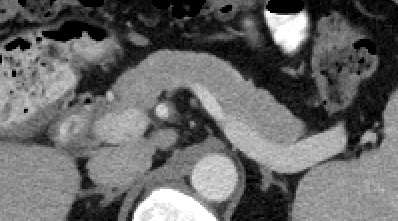
\includegraphics[width=0.20135\linewidth]{figures/panels/pancreas_ct_20pct_image} &
      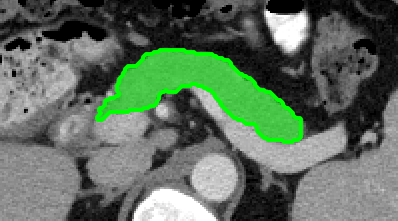
\includegraphics[width=0.20135\linewidth]{figures/panels/pancreas_ct_20pct_gt} &
      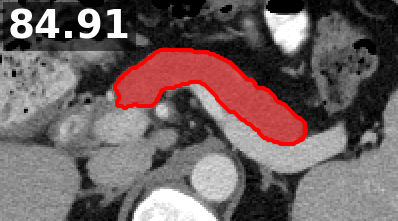
\includegraphics[width=0.20135\linewidth]{figures/panels/pancreas_ct_20pct_bcp} &
      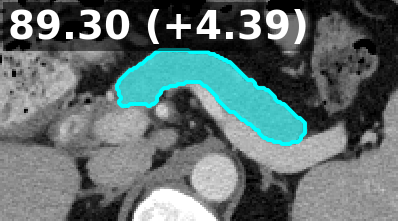
\includegraphics[width=0.20135\linewidth]{figures/panels/pancreas_ct_20pct_pem} \\
      \multicolumn{4}{c}{\footnotesize \textit{Pancreas-CT 20\%}} \\
      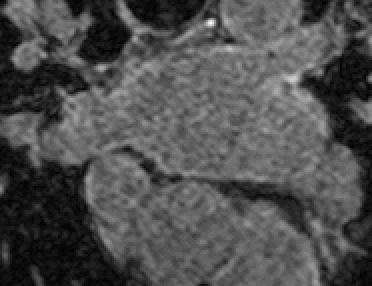
\includegraphics[width=0.20135\linewidth]{figures/panels/la_5pct_image} &
      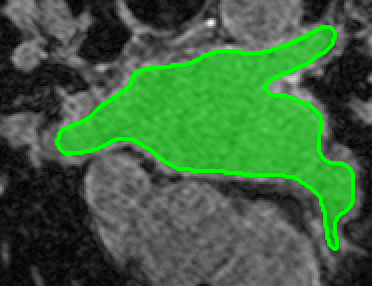
\includegraphics[width=0.20135\linewidth]{figures/panels/la_5pct_gt} &
      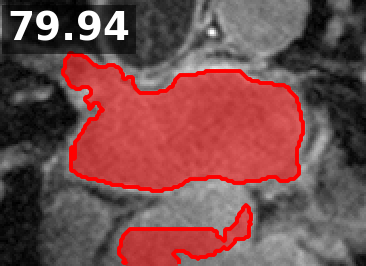
\includegraphics[width=0.20135\linewidth]{figures/panels/la_5pct_bcp} &
      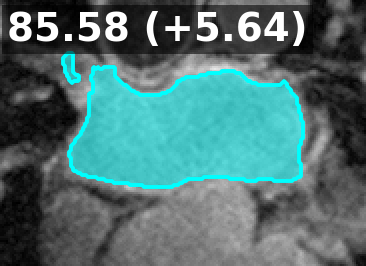
\includegraphics[width=0.20135\linewidth]{figures/panels/la_5pct_pem} \\
      \multicolumn{4}{c}{\footnotesize \textit{LA 5\%}} \\
      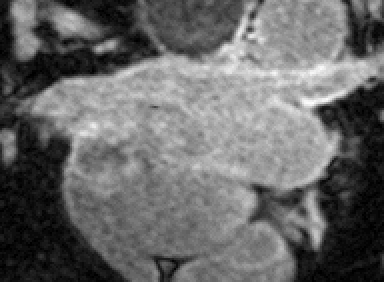
\includegraphics[width=0.20135\linewidth]{figures/panels/la_10pct_image} &
      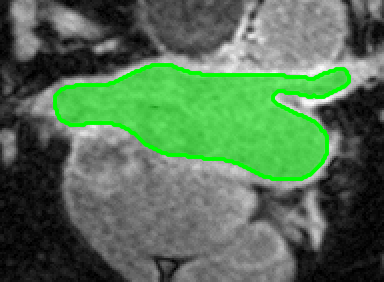
\includegraphics[width=0.20135\linewidth]{figures/panels/la_10pct_gt} &
      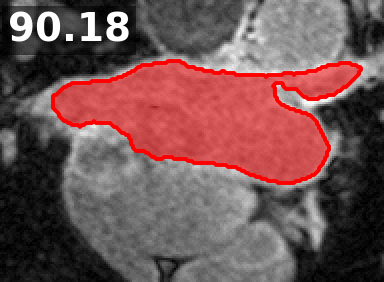
\includegraphics[width=0.20135\linewidth]{figures/panels/la_10pct_bcp} &
      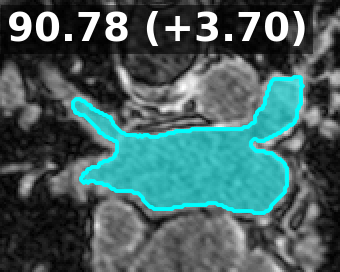
\includegraphics[width=0.20135\linewidth]{figures/panels/la_10pct_pem} \\
      \multicolumn{4}{c}{\footnotesize \textit{LA 10\%}} \\
    \end{tabular}%
  }
\vspace{-4pt}
\end{figure}

% ══════════════════════════════════════════════════════════════════════════════
\section{Discussion and Conclusion}
\label{sec:conclusion}
\vspace{-2pt}

PEM is a single-loss, training-free post-processing step that consistently improves both Dice ($+$0.9 to $+$1.6) and HD95 ($-$28\% to $-$44\%) on three benchmark configurations spanning two datasets, in under five minutes of fine-tuning.
It is complementary to stronger SSL training pipelines such as MOST~\cite{liu2024most} or DyCON~\cite{assefa2025dycon}: any SSL checkpoint exhibiting structured residual entropy can benefit, and we expect similar gains wherever such checkpoints become publicly available.

% \paragraph{Limitations.}
% PEM requires a well-converged base model and dataset-dependent learning-rate selection to avoid entropy collapse: a stronger base needs a gentler step.
% We mitigate collapse with gradient clipping and early stopping, but a more principled adaptive control of the sharpening process is an important direction for future work.

% \midlacknowledgments{We thank ethe reviewers for their valuable feedback.}

\bibliography{references}

\end{document}
